\documentclass[12pt]{article}
\usepackage{graphicx}
\title{Longest Increasing Sub-sequence \\in $O(NlogN)$ }
\author{MD. Sakib Khan}
\begin{document}
\maketitle
We have seen $O(N^2)$ solution of LIS(Longest Increasing Sub-sequence) using Dynamic Programming. Now we will see the $O(NlogN)$ solution using Searching Algorithm.\\
\\
Lets Say, We have an array(\textbf{Array[]}). We have to find the LIS of that array. For this, we will iterate the array from the first index and as much as the iteration done, we will save some result in an another array. (\textbf{LisTillNow[]}). Using that result we'll find the LIS. \\
\\
So in this way we'll follow two rules to get the LIS :
\begin{itemize}
  \item If all the values in \textbf{LisTillNow[]} is less than the   \textbf{Array[i]}, then we'll insert \textbf{Array[i]} at the end of the \textbf{LisTillNow[]} array.
  \item And if all the values in \textbf{LisTillNow[]} is not less than the \textbf{Array[i]} (Greater or equal), then the first value in \textbf{LisTillNow[]} which is greater than or equal to \textbf{Array[i]}, will be replaced by \textbf{Array[i]}.
\end{itemize}
Our main goal is to make the \textbf{LisTillNow[]} array Sorted and Longest.
\newpage
Let's see a simulation :
\Large{$$ Array[] = \{7,10,8,12,5,5,17,15\} $$}
\large{\textbf{\underline{Step 1:}}} 
$$
\begin{tabular}{|c|c|c|c|c|c|c|c|} \hline
     \Large{\textbf{7}} & & & & & & &  \\ \hline
\end{tabular} 
$$ \\
\normalsize{Though \textbf{LisTillNow[]} array is empty. so we simply insert 7 into that array.}. So, $$ \textbf{LisTillNow[] = \{ 7 \}} $$
\\
\large{\textbf{\underline{Step 2:}}} 
$$
\begin{tabular}{|c|c|c|c|c|c|c|c|} \hline
     7 & \Large{\textbf{10}} & & & & & &  \\ \hline
\end{tabular}
$$ \\
\normalsize{Though All the values in \textbf{LisTillNow[]} is less than \textbf{Array[1] = 10}, we simply insert 10 at the end of the array}. So, $$ \textbf{LisTillNow[] = \{ 7, 10 \}} $$
\\
\large{\textbf{\underline{Step 3:}}} 
$$
\begin{tabular}{|c|c|c|c|c|c|c|c|} \hline
      7 & 10 & \Large{\textbf{8}} & & & & &  \\ \hline
\end{tabular}
$$ \\
\normalsize{Though all the values in \textbf{LisTillNow[]} is not less than \textbf{Array[2] = 8}, So we have to find the first value in \textbf{LisTillNow[]} which is greater than or equal to 8, will be replaced by 8. We found 10 the first value which is greater than 8. we replace 10 by 8. So, } $$ \textbf{LisTillNow[] = \{ 7, 8 \}} $$
\newpage
\large{\textbf{\underline{Step 4:}}} 
$$
\begin{tabular}{|c|c|c|c|c|c|c|c|} \hline
     7 & 10 & 8 & \Large{\textbf{12}} & & & & \\ \hline
\end{tabular}
$$ \\
\normalsize{Like Step 2, we will insert \textbf{Array[3] = 12} at the at end of the \textbf{LisTillNow[]} array. So, } $$ \textbf{LisTillNow[] = \{ 7, 8, 12 \}} $$
\\
\large{\textbf{\underline{Step 5:}}} 
$$
\begin{tabular}{|c|c|c|c|c|c|c|c|} \hline
      7 & 10 & 8 & 12 & \Large{\textbf{5}} & & & \\ \hline
\end{tabular}
$$ \\
\normalsize{Like Step 3, we will replace 7 by \textbf{Array[4] = 5}. So, } $$ \textbf{LisTillNow[] = \{ 5, 8, 12 \}} $$
\\
\large{\textbf{\underline{Step 6:}}} 
$$
\begin{tabular}{|c|c|c|c|c|c|c|c|} \hline
      7 & 10 & 8 & 12 & 5 & \Large{\textbf{5}} & & \\ \hline
\end{tabular}
$$ \\
\normalsize{Like Step 3, we will replace 5 by \textbf{Array[5] = 5}. So, } $$ \textbf{LisTillNow[] = \{ 5, 8, 12 \}} $$
\\
\large{\textbf{\underline{Step 7:}}} 
$$
\begin{tabular}{|c|c|c|c|c|c|c|c|} \hline
      7 & 10 & 8 & 12 & 5 & 5 & \Large{\textbf{17}} & \\ \hline
\end{tabular}
$$ \\
\normalsize{Like Step 2, we will insert \textbf{Array[6] = 17} at the at end of the \textbf{LisTillNow[]} array. So, } $$ \textbf{LisTillNow[] = \{ 7, 8, 12, 17 \}} $$
\newpage
\large{\textbf{\underline{Step 8:}}} 
$$
\begin{tabular}{|c|c|c|c|c|c|c|c|} \hline
      7 & 10 & 8 & 12 & 5 & 5 & 17 &\Large{\textbf{15}}\\ \hline
\end{tabular}
$$ \\
\normalsize{Like Step 3, we will replace 17 by \textbf{Array[7] = 15} at the at end of the \textbf{LisTillNow[]} array. So, } $$ \textbf{LisTillNow[] = \{ 7, 8, 12, 15 \}} $$
And it is done. :) \\ \\ 
Following this way, we found a complete array \textbf{LisTillNow[]}. But it isn't a valid sub-sequence of the original array(\textbf{Array[]}). But the way, we get the \textbf{LisTillNow[]} array, the size of the \textbf{LisTillNow[]} array and the length of the LIS will be equal. We can easily prove that, $$ \textbf{LisTillNow[] = \{ 7, 8, 12, 15 \}} $$ Here, before 15, there must be a (3 length) Increasing Sub-sequence because before iterating \textbf{Array[7] = 15}, we had already found a (3 length) Increasing Sub-sequence. which is also true for 12.Before 12, there must be a (2 length) Increasing Sub-sequence because before iterating \textbf{Array[3] = 12}, we had already found a (2 length) Increasing Sub-sequence. Think a little bit, you will understand it clearly.\\
So, we have found the size of LIS, but how to find the original LIS array. Not to worry, slight modification of these process, can give you the original array.
\newpage
Now let's see how to code these things.\\
The main thing we need to do here is that, we have a value(\textbf{Array[i]}). We have to find a value which equal or immediate greater than (\textbf{Array[i]}). We can easily do it using \textbf{Binary Search} or we can use \textbf{lower\_bound()} Function of STL whose work is basically these, finding a value greater than or equal to a value in a sorted container.
\textbf{C++ Code:} \\ \\
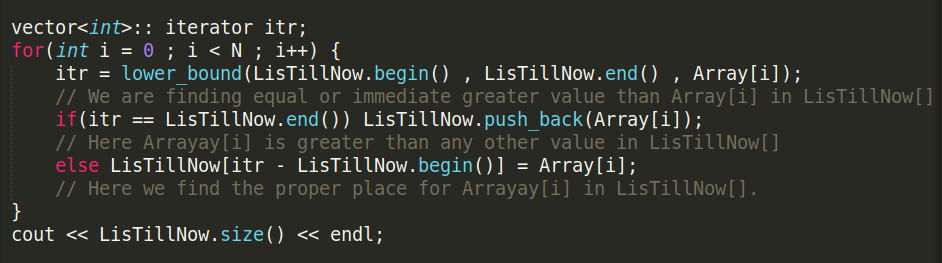
\includegraphics[width=\textwidth]{LIS} \\
To get the actual LIS array, we have to store another thing. When Placing \textbf{Array[i]} in \textbf{LisTillNow[]}, if we can store that index and the index of the value placed before \textbf{Array[i]} in \textbf{LisTillNow[]} Array, then we can simply get the original Array by traversing those indexes. \\ \\
\textbf{C++ Code:} \\ \\
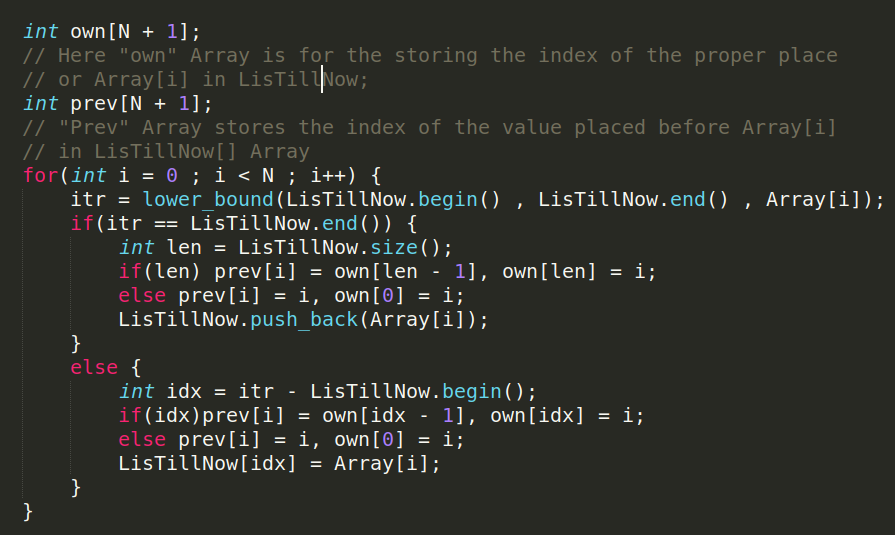
\includegraphics[width=\textwidth]{LOGN_print}
\newpage
How to Print The Path? Well, just traverse from the end (Stored index wise). \\ \\
\textbf{C++ Code:} \\ \\
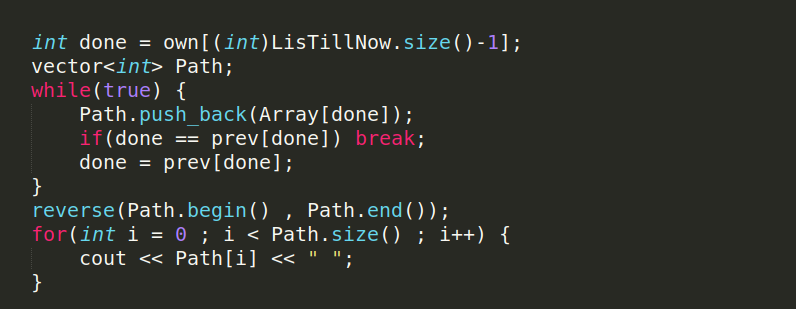
\includegraphics[width=\textwidth]{LOGN_PRINT_PATH}
\\ \\ 
\underline{\Large{\textbf{Some Variations of LIS:}}}
\begin{itemize}
\item Given an Array, You have to find \textbf{Longest Decreasing Sub-sequence} of that array. [Hints: Reverse the array. Now Find LIS] Also print The LDS array.
\item If LIS means Longest Increasing \textbf{(Not Strictly)}, Then Find the LIS of an array. [Hints: Use Upper\_bound() instead of lower\_bound()] Also Print the LIS array.
\item Find Maximum Sum Increasing Sub-sequence (If Maximum Sum is equal For two sub-sequence, find the longest sub-sequence) Also Print that Sub-sequence.
\item Given pair of numbers, Find LIS such that $A_i$ $<$ $ B_i $ and $A_j$ $<$ $ B_j $ where (i $<$ j)
\item Given pair of numbers, Find LIS such that $B_i$ $<$ $ A_j $ where (i $<$ j)
\item Find number of unique longest increasing sub-sequence in Array
\end{itemize}
Here is some UVA Online Judge Problems Based on LIS:- 111, 231, 437, 481, 497, 1196, 10131, 10534, 11368, 11456, 11790.
\end{document}